\chapter{介绍}

\section{托卡马卡及 EAST}
托卡马克是一类聚变磁约束装置,其环向场线圈产生特斯拉级别的约束磁场,而后等离子体中的电流产生了可以遏制极性漂移的极向场。环向场与极向场对约束起到了很关键的作用,且托卡马克的建设相对简单,其相关实验设备的参数在近数十年保持领先。

EAST (\textbf{E}xperimental \textbf{A}dvanced \textbf{S}uperconducting \textbf{T}okamak 实验先进超导托卡马克) 作为世界首个全超导托卡马克,多项参数取得领先,位于合肥等离子体物理研究所。
本文中的模拟均基于 \east 的 73999 序号实验,位型为上单零,具体见图 \ref{fig:equili-73999},可以观察到一定的不对称性。

\begin{table}[htb]
    \centering
    \caption{\east 设计参数}
    \label{tab:east_parameter}
    \begin{tabularx}{\linewidth}{lXlX}
        \toprule[1.5pt]
         & 参数 & & 参数\\
        \midrule[1pt]
        $R$ 大半径 &  \SI{1.7}{\meter} & $a$ 小半径 & \SI{0.4}{\meter}\\ 
        $B_t$ 环向中心磁感应强度 &  \SI{3.5}{\tesla} & 环径比 $R/a$ & $4.25$\\ 
        等离子体电流 $I_p$ & \SI{0.5}{\mega\ampere}&  &\\  % $\delta$ 三角形变系数
        \bottomrule[1.5pt]
    \end{tabularx}
\end{table}



\begin{figure}[htbp]
  \centering%
  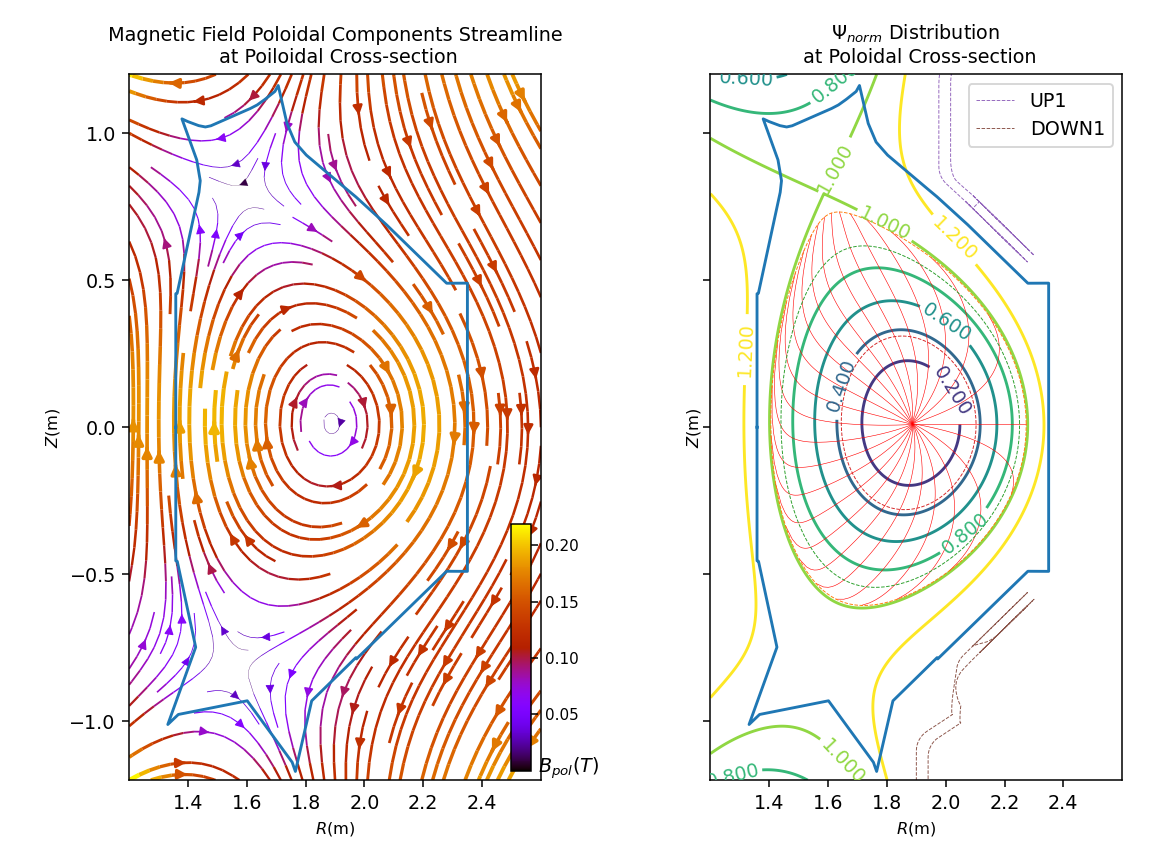
\includegraphics[width=1.00\columnwidth]{pol/pol.png}
  \caption{左图为极向切面下平衡场磁场的极向分量流线图,右图为 $\Psi_{norm}=s^2$ 分布,右图中还有 RMP 线圈的 UP1、DOWN1 线圈在 RZ 平面的投影。}
  \label{fig:equili-73999}
\end{figure}



托卡马克涉及到的磁流体不稳定性高度依赖于其边界磁面的螺旋形态。\textbf{旋转变换}(rotational transform, 本质上是磁面磁力线螺距角)的定义是磁力线绕环向方向转一圈时极向绕小半径转的圈数。假如磁面是互相嵌套的话,旋转变换在磁面上的平均值由极向磁通随环向磁通的变化率决定。
$ \iota/2 \pi = d\Psi /d \Phi $。

其倒数 \textbf{安全因子} 更常被使用,$q = 2\pi/\iota$。在截面圆形,主要由等离子体电流产生极向场的托卡马克中磁力线的方程近似满足 $ \frac{r d\theta}{B_\theta} = \frac{Rd\phi}{B_\phi} $,
其中 $ \phi $ and $\theta$ 分别是环向角和极向角。 于是在典型的托卡马克中, $ q = m/n = \left \langle d\phi /d\theta \right \rangle $ 可以用 $ q \simeq \frac{r B_\varphi}{R B_\theta} $ 近似。如果磁面安全因子 $q\leq 2$,边界上会发生显著的磁流体不稳定性。

在带偏滤器的托卡马克中,$q$ 在等离子体分界面趋近无穷,所以通常会考虑在分界面内侧的 $q$,通常来说会选 95\% 的磁面 (内部磁通占总环向磁通的 95\%), 此时常用 $q_{95}$ 来表示.





\section{边界局域模}
边界局域模 (Edge Localized Mode, ELM) 是一种在\Hmode 等离子体中存在的磁流体不稳定性,相比于\Lmode 等离子体,\Hmode 等离子体边界密度梯度和温度梯度更为显著,当梯度达到阈值时,等离子体边界会间歇性地将能量和粒子从边界脉冲式地释放出去,周而复始。\Hmode 最早在 ASDEX 托卡马克上被发现,其特点在于边界压强梯度较大,形成台基区(pedestal)。ELM 并不是完全不好,重复可控的边界局域模发生也可以帮助控制等离子体中的杂质存量。


边界局域模相关的理论难以给出能量和粒子损失速率的定量描述,于是便很难和实验的对比。可以比较的是实验观测到的时间尺度,例如,边界局域模的上升时间尺度,持续时间尺度以及在以及边界局域模重复频率的变化趋势,另外,边界局域模发生的径向范围可以用理论给出,这可以和实验的发现进行一个对比。ELM 在 \ddd、ASDEX 等装置上得到了充分的研究,根据许多托卡马克装置上的实验对其特征进行了下面的归纳,Zohm \cite{zohm_edge_1996} 将其划分为三类,其中振荡循环型是 L-H 转换过渡期发生的。


\begin{itemize}
    \item \textit{\typeone ELM}  \\ 重复频率 $\nu_{ELM}$ 随着加热功率的增加而增加。在高温时,理想气球模限制了可以达到的边界最大压力梯度 $\alpha/\alpha_{\text{crit}}\approx 1$,并耦合了低 $n$ 的剥离模,\typeone ELM 就会发展起来。\\
    这种类型的 ELM 在目前的实践中,没有显著的磁前兆振荡被检测到,不过发生之前会有密度湍流波动的增强,且会使得 $D_\alpha$ 信号产生间断的剧烈爆发。
    \item \textit{\typethr ELM} \\ 重复频率 $\nu_{ELM}$ 随着加热功率的增加而减小。在 L-H 转换之后,在边界的电子温度不太高的情况下,等离子体边界压力梯度显著低于理想气球模的极限,即 $0.3\leq \alpha/\alpha_{\text{crit}}\leq 0.5$。随着输入功率增高,足够高的温度使阻尼效应可忽略时,\typethr ELM 会一定程度被缓解。
\end{itemize}

在 L-H 转换过程中也会发生一种现象,称为 \textit{Dithering Cycles, 振荡循环型} ELM。由于\Hmode 功率的滞后而在阈值上下而往复的循环是有可能的。边界的压力和电流梯度和 \Lmode 时类似,所以可以说,振荡周期型不是一种典型的磁流体不稳定性,而是一种 L-H-L 模转换连续发生的现象。

尽管受 ELM 复杂的非线性物理所限,这样的描述不能作为一种 ELM 的精确定义。但这种唯象的理解是基于实验观测到的结果,并且和目前对磁流体稳定性的分析相差不甚。



Loarte 等\cite{2003PPCF...45.1549L} 基于目前装置上实验参数的外推结果,\iter 上 \typeone ELM 可能会导致损失 $5\sim \SI{22}{\mega\joule}$ ,其中约一半分布在 $\sim \SI{1}{\meter^2}$ 壁上的热沉积范围\inlinecite{Loarte_2014}。壁材料瞬态接受的能量密度在 $2.5\sim \SI{11}{\mega\joule/\meter^2}$,是目前材料(钨或碳纤维材料)承受热负荷能力的 $5\sim 20$ 倍。通过何种手段缓解或抑制 ELMs 成为了相当关键的一个问题,而由共振磁扰动(RMP)引起的边界随机场实验验证是一种可以有效缓解或抑制 \typeone 大 ELM 的有效方法。


但这种作用过程是复杂的,等离子体对共振磁扰动会产生较强的响应以屏蔽扰动场磁谱中的共振分量,大大地降低共振扰动磁场对等离子体边界磁拓扑随机化影响的程度\inlinecite{sun_nonlinear_2016},这使得通过扰动场施加共振磁扰动以有效可靠地抑制边界局域模 ELM 的机制还需要深入的研究。这种复杂程度还体现在,目前对 ELM 的缓解和抑制之间的关键区别还不明晰,等离子体对 ELM 抑制的线性/非线性响应均有待探索。

\section{扰动场}

在聚变等离子体中用到的外加扰动场(magnetic perturbation, MP)是指螺旋形或鞍形线圈产生的量级为 $\delta B_r/B_t=10^{-5}\sim 10^{-3}$ 的磁场扰动。将外加磁扰动的径向分量在磁面坐标系中进行二维 Fourier 运算,可以得到其磁谱,对应不同的环向模数 $n$ 和极向模数 $m$。磁谱中 $m,n$ 的分量与安全因子为 $q_s=m/n$ 的有理面会形成共振,在该磁面施加的径向磁场螺旋度和平衡场的一致,从而可以对有理面上的不稳定性造成较大影响。因此,磁扰动中的这些分量特别地命名为共振磁扰动(Resonant Magnetic Perturbation, RMP)。


RMP 使得其在某个特定的磁面产生磁岛链(通常指等离子体边界区域),研究人员希望通过 RMP 实现等离子体边界磁拓扑的随机化,从而缓解或抑制 ELM,避免脉冲式的粒子流和热负荷,使得直面等离子体的材料能够长时间工作。下面介绍在本文中涉及到的产生磁扰动的线圈和电流丝。


\subsection{低 n 线圈}
低 n 线圈传统上称为 RMP 线圈,2014 年在 EAST 的低场侧安装了一套,它包含有两组线圈($2*8=16$)。EAST 团队通过扰动场环向模数为 $n=1, 2$ 的 RMPs 实现了 \typeone 边界局域模的缓解和完全的抑制。我们在正文中的模拟部分将会看到,低环向模数的工作模式会有较好的生成随机场的效果,高环向模数主导 $n>2$ 的工作模式则有所不及。

  
\begin{figure}[htbp]
  \centering%
      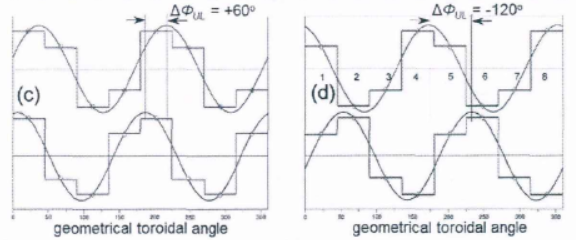
\includegraphics[width=0.8\columnwidth]{lown/lown_coil_current_phase.png}
      \caption{J-TEXT 上 RMP 线圈通电电流和相位的关系,图中 (c) 和 (d) 显示了两个不同相位差的时候环向上线圈电流分布}
      \label{fig:lown_current}
\end{figure}


一般而言低 n 线圈中电流由其想要产生的环向模数和相位所决定,

\begin{equation}
I(\varphi)=I_{\max } \times \cos \left(n \varphi-\Phi_{i}\right)
\end{equation}

其中 $\Phi_i, i\in \{U,L\}$ 表示上下沿线圈的电流基准相位,配合各线圈所在的环向角度 $\varphi$ 在不同线圈上给出不同的电流幅值。

\begin{equation}
\Delta \Phi_{UL} = \Phi_U - \Phi_L
\end{equation}

根据实际的线圈电源的接口配置,可以有更任意的电流大小选取,但一般而言上述三角函数式的电流大小设置足够以产生较好的扰动效果。

\subsection{高 m 线圈}
等离子体所新近研发的高 m 线圈 \inlinecite{zhang_highm} 激发出的扰动场有着高 m,宽 n 特征,分为上下对称两组($2*2=4$),最大额定电流为 \SI{5}{\kilo\ampere},工作电流可随时间变化。 
物理计算过程中采用的线圈几何尺寸如图 \ref{fig:highm-pos} 所示。由于高 $m$ 线圈组设计位于一个极向截面内,即 $\phi\equiv \text{const}$ 处,其对等离子体的影响局域性很明显,此类强局域性扰动磁场对等离子体边界稳定性的影响可以从中得到研究。

高 m 线圈采用与现有 RMP 线圈系统相同的线圈材料,线圈位置位于低场侧限制器后方,利用限制器作为线圈的保护,从而可尽可能地靠近等离子体。根据两组线圈内电流的相对方向,有两种工作模式,见图 \ref{fig:highm-pos}。\textit{主要工作模式}时两组线圈通同向电流;\textit{次要工作模式}时则反向。


\begin{figure}[htbp]
    \centering%
    % \hspace{4em}%
    \begin{subfigure}{0.45\textwidth}
      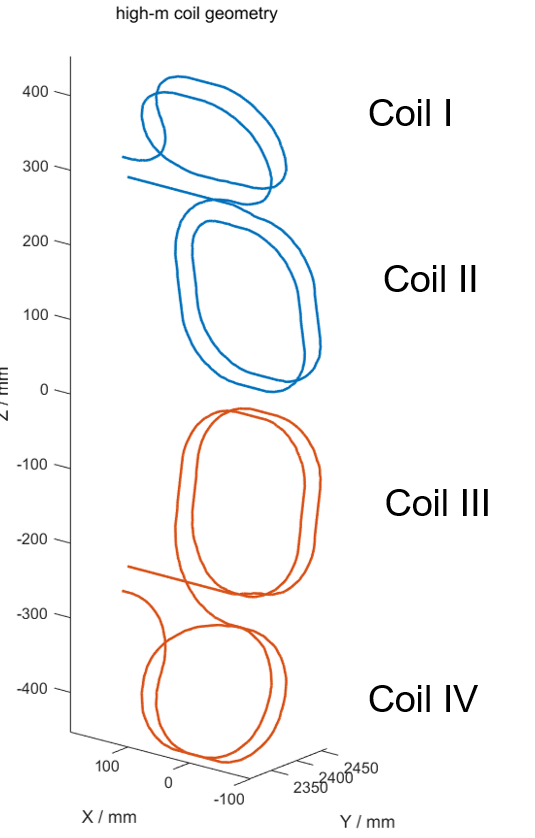
\includegraphics[height=8cm]{highm/coil_geometry.png}
      \caption{高 $m$ 线圈的立体几何位置}
    \end{subfigure}
    % \hspace{4em}%
    \begin{subfigure}{0.45\textwidth}
      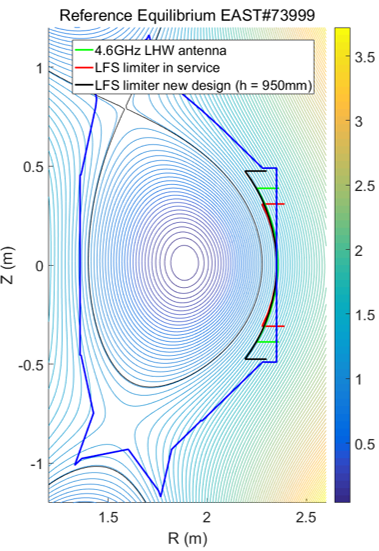
\includegraphics[height=8cm]{highm/coil_limiter_pos.png}
      \caption{极向截面上高 $m$ 线圈的位置}
    \end{subfigure}
    \caption{高 $m$ 线圈在 \east 中的设计和所处的几何位置,源自 \cite{zhang_highm}}
    \label{fig:highm-pos}
  \end{figure}










\subsection{低杂波驱动的螺旋电流丝}
RMP 致命的弱点是线圈置于装置真空室内,这在 DEMO 堆中会带来较高的工程难度和安全风险,研究人员正在积极探索通过其他手段来改变边界磁拓扑。 利用低杂波在等离子体边界刮削层内获得的螺旋电流丝,是一个很有吸引力的在下一代聚变设备中应用的 RMP 手段。


\begin{figure}[t]
  \centering
  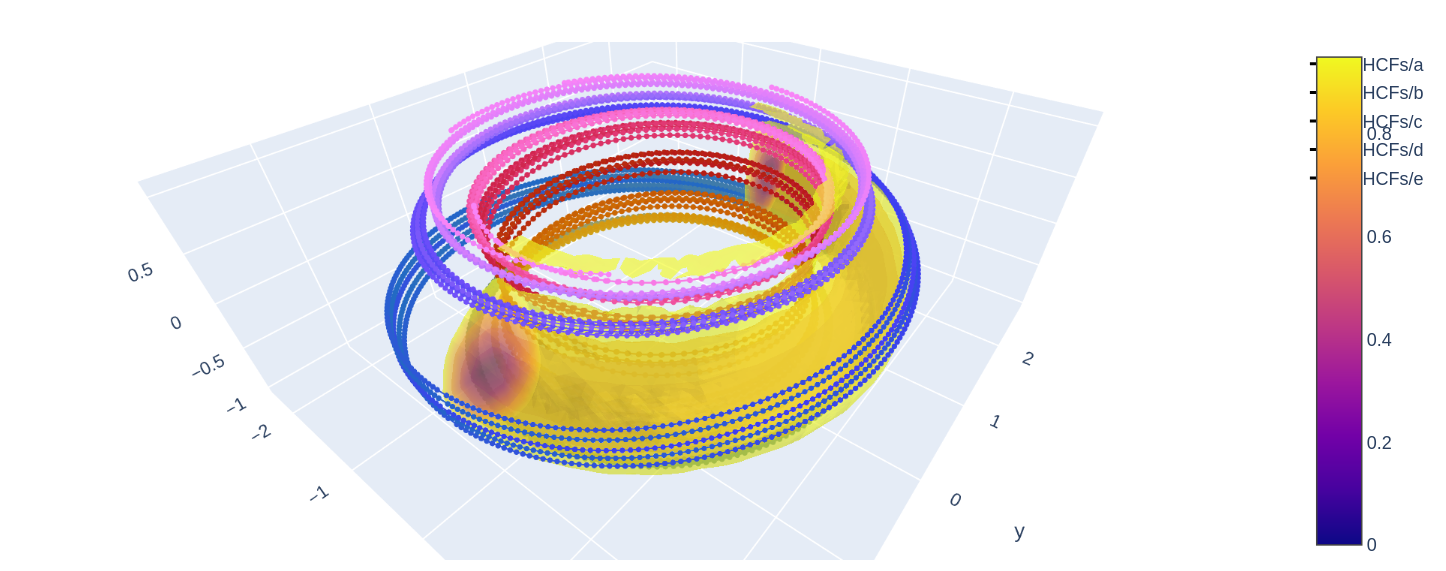
\includegraphics[width=0.9\columnwidth,keepaspectratio]{73999_030400ms_improved/hcfs_east.png}
  \caption{基于磁力线追踪计算得到的螺旋电流丝轨迹,五条分别螺旋电流丝起点分别取为五排低杂波天线的中间位置正对着的闭合磁面外 10 mm。}
  % Helical Current Filaments induced by LHW
\end{figure}

低杂波加热原本用于芯部等离子体电流驱动,它通过朗道阻尼将动量传给等离子体,可以实现完全非感应电流的长脉冲\Hmode 运行。但在加热作用之外,还在 \east 等装置上发现了低杂波驱动的螺旋电流丝,低杂波启动后毫秒内电流丝即响应出现,电流丝数量和托卡马克中低杂波天线的行数相同。


在 EAST 中为了研究低杂波及螺旋电流丝,以氦气放电实验来用可见光显著地表现螺旋电流丝的三维几何分布可见附录;以方波调制的低杂波功率进行了间断性的螺旋电流丝激励 \inlinecite{the_east_team_magnetic_2013}。低杂波系统运转时,螺旋电流丝引起的三维磁拓扑变化导致了粒子流在偏滤器平板上形成了三维特征的分裂模式\cite{the_east_team_magnetic_2013}。



% \section{\Poincare 图及傅里叶模数分析}
% \Poincare 图是对磁面结构的描述,通过在给定极向截面上进行沿磁力线的迭代来标记在同一磁面上的点,以描绘出磁面的嵌套结构。

% \subsection{质点网格法 Particel-in-cell (PIC)}

% 在以上的偏微分方程求解时,物理问题允许将某一点(或一个邻域内)的物理量取其代表值来离散化,如有限体积法中取其网格内的平均值进行计算,,有限元法中取有限阶多项式逼近。然而,在并不一定完全服从高斯速度分布的等离子体物理研究中,这样的代表值很难抽取出来。类似的非高斯型速度分布导致的流体假设不成立的问题,在裂变堆中子物理计算中采用的是多群计算的方法;而在聚变等离子体物理问题中,不论是自然产生的等离子体还是人工产生的加速器,往往会出现相当各向异性的速度分布,以至于需要细致地考虑在相空间中求解。对粒子在相空间(Phase space)中的分布函数 $f(\vec{x},\vec{v},t)$,描述其演化规律的物理方程是 Boltzmann 方程,\cite{ColonnaBoltamann10.1088/978-0-7503-1200-4ch1}.

% \begin{equation}
% \label{eq:Boltzmann}
% \frac{\partial f_{s}(\vec{r}, \vec{v}, t)}{\partial t}+\left[\vec{v} \cdot \nabla_{r}+\vec{a}(\vec{r}) \cdot \nabla_{v}\right] f_{s}(\vec{r}, \vec{v}, t)=\left(\frac{\delta f_{s}}{\delta t}\right)_{\mathrm{coll}}
% \end{equation}

% 其中 $(\delta f_{s}/\delta t )_{\mathrm{coll}}$ 表示同种粒子及不同粒子之间的相互碰撞导致的粒子 s 的 $f_s$ 变化率。
% Particle-in-cell, 即 PIC 手段将电磁场进行常规的偏微分方程求解,另外,还令网格中分布着巨粒子。巨粒子对网格角点处的电磁场参数数值有所影响,同时巨粒子也会根据离散的电磁场计算其下一时间步长的速度和坐标,这样就一定程度上在完全的粒子模拟和有限网格计算方法之间达到所需要的性能、准确之间的平衡。

​\section{主要目标}
为了探究解决目前的\Hmode 等离子体所面临的 ELM 脉冲式热流和粒子流问题,\iter 设计为工作在\Hmode 状态但其如此强烈的脉冲式载荷却是在正式运行时是不允许的。
为更好地控制 ELM, EAST 上先后测试了共振磁扰动线圈 RMP、高 m 线圈和低杂波驱动的螺旋电流丝,这三种扰动场产生机制有所差异,适用的范围也不尽相同。为了使扰动场相互配合达到最优的缓解乃至抑制边界局域模的效果,对它们协同作用的研究是很有必要的。

\textit{\textbf{(1)}} \textbf{低 $n$ 线圈},该线圈布置在真空室内,由它激发起环向模数为 $n=1,2$ 的扰动场后在 \east, \ddd 等托卡马克装置上验证了其抑制边界局域模的效应。 
\textit{\textbf{(2)}} \textbf{高 m 线圈},是 EAST 团队近两年设计中的线圈,在等离子体环外加上一组四个的线圈,它的特征是扰动场环向模数 n 分布较宽,极向模数 m 较高,由于只分布在一个环向位置 $\varphi=\text{const}$,扰动场的局域性很强。 
\textit{\textbf{(3)}} \textbf{螺旋电流丝}(由低杂波驱动),低杂波原本用于以朗道阻尼驱动芯部等离子体的电流,但在设计之外,实验发现它在等离子体边界会激发出螺旋电流丝,电流丝产生具体的物理机制还不甚明晰,但其亦具备调节边界磁拓扑的能力。由于低杂波天线不像共振磁扰动线圈在腔内,它具有应用在 DEMO 堆及日后商业堆的潜力。

第二章首先给出几种扰动场的主要磁谱特征,对磁扰动场径向分量在磁面 Fourier 分析得到的磁谱 $\tilde{b}^1_{mn}$ 和 \Poincare 图。第三章进入本文主体,线圈之间如何配合以能够对等离子体施加合适的磁扰动场,为此。这一章的主体是通过扰动场之间的配合达到较好的抑制 ELM 及保持芯部等离子体较好约束的效果。进一步在第三章中将讨论不同扰动场的配置下第一壁材料上的热负荷和粒子流分布。尽管主要依赖于对 ELM 的抑制效果来选择磁扰动场,但基于扰动场的热负荷优化分布或时间调制能够给出了一种新的调节视角。对下一代托卡马克而言,\Hmode 等离子体会造成难以承受的热流和粒子流,扰动场可以提供一种调节 ELM 的手段,避免脉冲式的 ELM 破裂造成的材料损害。

本文着重以模拟的手段对现有的多种三维磁场进行模拟仿真,它们的磁谱被设计用来缓解或者调节边界局域模的发生。但同时也研究给定扰动场对粒子束流和热流的调节作用。
